\section{Potentiale}\label{sec:Potentiale}

\subsection{Definitionen}

\begin{defn}
	Eine Funktion $P: X \to \IR$ heißt\todo{Verallgemeinern? (total geordnete Menge $K$ statt $\IR$?)}
	\begin{itemize}
		\item \emph{Beste Antwort-Potential}, wenn für jeden Spieler $i$ und alle Strategieprofile $x_{-i} \in X_{-i}$ gilt:
			\[\arg \min_{x_i \in X_i}c_i(x) = \arg \min_{x_i \in X_i} P(x)\]
		\item \emph{verallgemeinertes ordinales Potential}, wenn für jeden Spieler $i$ und alle Strategieprofile $x_{-i} \in X_{-i}$ sowie $x_i, \hat{x}_i \in X_i$ gilt:
			\[c_i(x_i,x_{-i}) > c_i(\hat{x}_i, x_{-i}) \implies P(x_i,x_{-i}) > P(\hat{x}_i, x_{-i})\]
		\item \emph{ordinales Potential}, wenn für jeden Spieler $i$ und alle Strategieprofile $x_{-i} \in X_{-i}$ sowie $x_i, \hat{x}_i \in X_i$ gilt:
			\[c_i(x_i,x_{-i}) > c_i(\hat{x}_i, x_{-i}) \iff P(x_i,x_{-i}) > P(\hat{x}_i, x_{-i})\]
	\end{itemize}
	Sind die $K_i$ zudem geordnete abelsche Gruppen, so heißt $P$
	\begin{itemize}
		\item \emph{skaliertes Potential}, wenn es streng monotone Funktionen $f_i: \IR \to K_i$ gibt, die $0$ auf $0$ abbilden, sodass für jeden Spieler $i$ und alle Strategieprofile $x_{-i} \in X_{-i}$ sowie $x_i, \hat{x}_i \in X_i$ gilt:
			\[c_i(x_i,x_{-i}) - c_i(\hat{x}_i, x_{-i}) = f_i(P(x_i,x_{-i}) - P(\hat{x}_i, x_{-i}))\]
	\end{itemize}
	Sind die $K_i$ Teilmengen eines gemeinsamen geordneten Rings $K$, so heißt $P$
	\begin{itemize}	
		\item \emph{gewichtetes Potential}, wenn es einen Gewichtsvektor $(w_i)_{i\in I}$ gibt, sodass für jeden Spieler $i$ und alle Strategieprofile $x_{-i} \in X_{-i}$ sowie $x_i, \hat{x}_i \in X_i$ gilt:
			\[c_i(x_i,x_{-i}) - c_i(\hat{x}_i, x_{-i}) = w_i\cdot(P(x_i,x_{-i}) - P(\hat{x}_i, x_{-i}))\]
		\item \emph{exaktes Potential}, wenn für jeden Spieler $i$ und alle Strategieprofile $x_{-i} \in X_{-i}$ sowie $x_i, \hat{x}_i \in X_i$ gilt:
			\[c_i(x_i,x_{-i}) - c_i(\hat{x}_i, x_{-i}) = P(x_i,x_{-i}) - P(\hat{x}_i, x_{-i})\]
	\end{itemize}
\end{defn}\todo{Kann man diese Definition irgendwie kompakter/übersichtlicher machen?}

Exakte, gewichtete, ordinale und verallgemeinerte ordinale Potentiale wurden erstmals in \cite{MonShap} definiert, beste Antwort-Potentiale erstmals in \cite{BestRespPot}.

\subsection{Anschauung}

In einem gewissem Sinne definiert jedes Potential ein alternatives Spiel mit gleichem Strategieraum, aber einer anderen, für alle Spieler einheitlichen Kostenfunktion (nämlich der Potentialfunktion). In einem solchen Spiel ist es nun viel einfacher beispielsweise Gleichgewichts- oder Optimalitätspunkte zu finden (da hierzu nur eine einzige Funktion betrachtet werden muss). Eigenschaften, die beim Übergang zurück zum ursprünglichen Spiel erhalten bleiben, kann man dann einfach in dem einfacheren Spiel überprüfen. Diesen Übergang werden wir später mit Hilfe von (Iso-)Morphismen formal fassen (siehe \Cref{sec:Morphismen}).

Hier wollen wir nun noch kurz darauf eingehen, wie sich die verschiedenen Potentialbegriffe anschaulich untereinander unterscheiden. Wir betrachten dazu (endliche) 2-Personenspiele. Deren Strategieraum kann man dann als Gitternetz in der Ebene auffassen, wobei jede Strategie von Spieler 1 einer senkrechten und jede Strategie von Spieler 2 einer waagerechten Gitterlinie entspricht. Kreuzungspunkte von zwei Gerade entsprechen dann gerade vollständige Strategieprofilen. Kostenfunktionen (ebenso wie Potentiale) sind dann \glqq Reliefkarten\grqq{}, deren Höhe den jeweiligen Kosten entspricht. 

\begin{figure}[h]\centering
	\includegraphics[width=.3\textwidth]{../Bilder/exaktesPotentialSp1.pdf}
	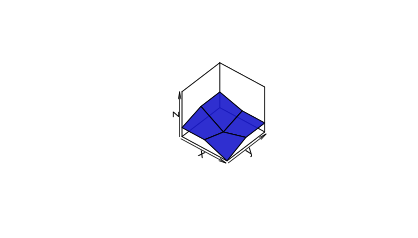
\includegraphics[width=.3\textwidth]{../Bilder/exaktesPotentialSp2.pdf}
	\includegraphics[width=.3\textwidth]{../Bilder/exaktesPotential.pdf}
	\caption{Ein 2-Personenspiel mit exaktem Potential (grau): Spieler 1: rot, Spieler 2: blau}
\end{figure}

Ein exaktes Potential entspricht dann einer gemeinsamen Reliefkarte für beide Spieler, die - im Falle eines exakten Potentials - \glqq scheibenweise\grqq{} bis auf eine additive Konstante mit der eigentlichen Kostenfunktion übereinstimmt. Anders formuliert: Wird dies Strategie eines Spieler festgehalten, so kann der andere Spieler seine Kostenveränderungen bei der Wahl der verschiedenen ihm zur Verfügung stehenden Strategien auch anhand der Potentialfunktion ablesen. 

Geht man nun über zu einem gewichteten Potential, so lesen die beiden Spieler das Potential sozusagen in verschiedenen Einheiten\todo{eigentlich müssen verchiedene Einheiten nicht zwangsläufig proportional zueinander sein - für Längeneinheiten sollte es typischerweise aber stimmen}. Das heißt die Kostenveränderungen eines Spielers sind nur noch proportional zu den Potentialänderungen. Ein skaliertes Potential zeigt jedem Spieler noch an, welche der Kostenveränderungen eher groß und welche klein sind. Ordinale Potentiale zeigen nur noch die Richtung der Kostenveränderung an (\glqq wird teurer\grqq / \glqq wird billiger\grqq / \glqq Kosten bleiben konstant\grqq) und verallgemeinerte ordinale Potentiale zeigen nur noch echte Steigungen korrekt an. Beste-Antwort-Potentiale schließlich zeigen immer die beste Antwort an.


\todo[inline]{Zusammenhänge (evtl. schon nächstes Kapitel?)}

Eine Beobachtung aus \cite{CharExGewPotinWCG}:

\begin{beob}\label{beob:ZshExGewPot}
	Ein Spiel $\Gamma = (I, (X_i)_{i \in I}, (c_i)_{i \in I})$ besitzt genau dann ein gewichtetes Potential (mit Gewichtsvektor $(w_i)_{i \in I}$), wenn $\Gamma' := (I, (X_i)_{i \in I}, (w_i \cdot c_i)_{i \in I})$ ein exaktes Potential besitzt.
\end{beob}

Folgt auch aus einer allgemeineren Beobachtung in \Cref{sec:Morphismen}.

\subsection{Erste Sätze}

Zu einem gegebenen Strategieprofil $x \in X$ sei dessen \emph{Nachbarschaft} die Menge aller durch höchstens eine Abweichung erreichbarer Strategieprofile, d.h. die Menge $\{(\hat{x}_i, x_{-i}) | i \in N, \hat{x}_i \in X_i\}$. Wir nennen $x$ dann ein \emph{lokales Minimum} einer Funktion $f: X \to \IR$, wenn es ein Minimum innerhalb seiner Nachbarschaft ist.

\begin{satz}\label{satz:lokMinNG}
	Sei $\Gamma$ ein Spiel mit einem verallgemeinerten ordinalen Potential $P$. Dann ist jedes lokale Minimum von $P$ ein Nash-Gleichgewicht von $\Gamma$. Ist $P$ sogar ein ordinales Potential, so gilt auch die umgekehrte Richtung.
\end{satz}

\todo[inline]{Diese Sätze hier evtl. nur erwähnen und erst später (nach der Definition von Morphismen) formalisieren (und beweisen)}

Dieser Satz zeigt also, dass man Nash-Gleichgewichte allein durch Betrachten einer Potentialfunktion finden kann. Daraus  folgt direkt die Existenz von Nash-Gleichgewichten in einer Vielzahl von Potentialspielen:

\begin{kor}
	Sei $\Gamma$ ein Spiel mit einem kompakten Strategieraum und einer stetigen verallgemeinerten ordinalen Potentialfunktion. Dann hat $\Gamma$ wenigstens ein Nash-Gleichgewicht.
\end{kor}

Insbesondere also haben endliche Potentialspiele immer ein Nashgleichgewicht. \Cref{satz:lokMinNG} folgt mit Hilfe von \Cref{kor:ExVerbPfadExNG} direkt aus dem folgenden Satz\todo{Streng genommen nicht wirklich, da das Korollar nur für Spiele gilt!?}:

\begin{satz}
	Sei $\Gamma$ ein Spiel mit einem verallgemeinerten ordinalen Potential $P$. Dann ist jeder Verbesserungspfad in $\Gamma$ auch ein Verbesserungspfad bezüglich $P$. Ist $P$ sogar ein ordinales Potential, so gilt auch die umgekehrte Richtung.
\end{satz}

\begin{proof}.
	
	\todo[inline]{Beweis}	
\end{proof}

\todo[inline]{Was kann man über Beste-Antwort-Potentiale sagen (vermtl. Zusammenhang zu Beste-Antwort-Pfade?)}


\subsection{Charakterisierungen der Potentiale}

\begin{satz}
	Ein Spiel besitzt genau dann ein exaktes Potential, wenn alle 4-Zykel im Strategieraum eine Gesamtänderung von $0$ haben.
\end{satz}

\begin{proof}.
	
	\todo[inline]{vgl. \cite[Theorem 2.8]{MonShap}}
\end{proof}

\begin{satz}
	Ein Spiel besitzt genau dann ein gewichtetes Potential, wenn ... \todo{analoge Bedingung zu exaktem Potential (vgl. \cite[Kapitel 3.2]{CharExGewPotinWCG})}
\end{satz}

\begin{proof}.
	
	\todo[inline]{mit \Cref{beob:ZshExGewPot}?}
\end{proof}

\begin{satz}
	Ein Spiel besitzt genau dann ein ordinales Potential, wenn es keine schwachen Verbesserungskreise enthält und $([X], <)$ properly ordered\todo{Fehlt Definition} ist.
\end{satz}

\begin{proof}.
	
	\todo[inline]{aus \cite{CharExOrdPot}}
\end{proof}


\begin{satz}
	Hat ein Spiel die FIP, so besitzt es auch ein verallgemeinertes ordinales Potential.
	
	Umgekehrt besitzt jedes \emph{endliche} Spiel mit einem verallgemeinerten ordinalen Potential auch die FIP.
\end{satz}

\begin{proof}
	\cite{MonShap}/\cite{CongGamesPlayerSpecPayoff} (konstruktiver Beweis)
\end{proof}

\begin{satz}
	Ein Spiel hat genau dann ein Beste Antwort-Potential, wenn es keine beste-Antwort-kompatiblen Kreise enthält und $([X], <)$ properly ordered ist.
\end{satz}

\begin{proof}.
	
	\todo[inline]{aus \cite{BestRespPot}}
\end{proof}